\chapter{Introduction}
\chapter{Literature Review}

\textcolor{red}{To the literature review, I also want to add a section 
discussing the research on societal risk and risk acceptability. E.g., F-N
curves.}

\textcolor{red}{To the literature review, I want to add a section discussing 
the research on modeling at the municipal level. These papers start with the 
following: 
\cite{mckenna_combining_2018,johannsen_municipal_2023,ben_amer_too_2020}.}

\chapter{\acf{osier}}
\label{chapter:osier}

This chapter introduces \acf{osier}, a novel open-source energy system modeling
framework for \acl{moo} \cite{dotson_osier_nodate}. There are currently no
\acp{esom} that enable \ac{moo} and \ac{osier} fills that gap. Figure
\ref{fig:osier_flow} illustrates the flow of data into and within \ac{osier}.

\begin{figure}[H]
    \centering
    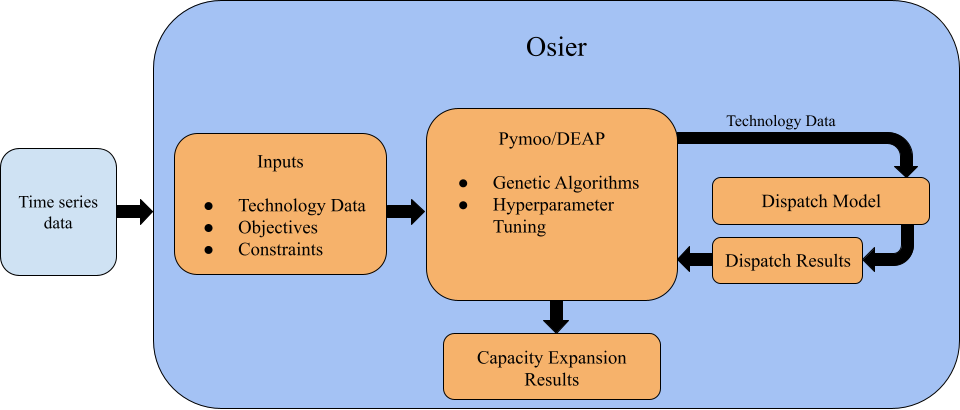
\includegraphics[width=\columnwidth]{figures/osier_flow}
    \caption{The flow of data into and within \ac{osier}}
    \label{fig:osier_flow}
\end{figure}

Technology data, objectives, constraints, and a dispatch model are all features
within \ac{osier}, while \ac{pymoo} drives the optimization of these objectives.
The dispatch model is independently executable for inspecting specific test
cases and mapping solutions from other solvers onto \ac{osier}'s objective
space. The next section elaborates on the dispatch model's formulation.

\textcolor{red}{This chapter is mostly written but there are a few things that
should be added.}

\textcolor{red}{\begin{enumerate}
    \item Update to the \ac{mga} algorithm.
    \item Add description of the ``greedy'' farthest-first traversal algorithm.
    \item Move the description of \ac{pygen} and \ac{temoa} to either a
    different section or a different chapter since those pieces do not belong to
    \ac{osier} itself.
    \item Add a description of the ``simplified approach'' to capacity expansion
    that will be added to the model and used the example chapter.
    \item Remove the description of model data.
    \item Add a description of the hypothetical \ac{osier} procedure, as
    proposed in the prelim.
\end{enumerate}}

\section{Inputs}

\textcolor{red}{General thoughts:}

Accurate input data is essential but represents a challenging step in the
modeling process. \ac{osier} attempts to lower this barrier by providing a
variety of technology data from ``reliable'' sources.

This section connects to the normative and descriptive portions of modeling. 

\subsection{Technology Data}

\subsection{Objectives}

\subsection{Constraints}

\section{Genetic Algorithms}

\section{Dispatch Model}

\subsection{Economic/Merit-order dispatch}

\subsection{Simplified dispatch}


\chapter{Benchmark Results}
\label{chapter:benchmark-results}

\textcolor{red}{This chapter will remain largely unchanged except for maybe one
additional example, demonstrating a different dispatch model that is much faster
but less robust. This new dispatch model will be used in the following chapter
where I investigate further examples including a hypothetical ``data center''
and an improvement on the \acf{set} \cite{wigeland_nuclear_2014}.}

\section{Exercise 0: Deciding Among Evolutionary Algorithms}

\textit{Already written in prelim document.}

\section{Exercise 1: Exploring objective space}

\textit{Already written in prelim document.}

\section{Exercise 2: Four Simultaneous Objectives}

\textit{Already written in prelim document.}

\section{Exercise 3: Validating a Simplified Approach}

\textcolor{red}{This section is new in the dissertation.}

\chapter{Examples with \acs{osier}}
\label{chapter:examples}

\textcolor{red}{This chapter is entirely new to this thesis!}

\section{Example 1: Updating the \ac{set}}

\subsection{Overview of the Nuclear Fuel Cycle}

\subsection{What is the \ac{set}?}

\subsection{What metrics are available?}

\subsection{Data for the simulation}

\subsection{Results}

\subsection{Discussion}

\section{Example 2: Powering a Data Center}

\subsection{Why data centers?}

\subsection{What technology options exist?}

\subsection{Data for the simulation}

\subsection{Results}

\subsection{Discussion}

\chapter{Using modeling to enhance just outcomes}

This chapter addresses my proposal to ``validate'' \ac{osier} by conducting a
case study of energy planning processes in Champaign-Urbana through interviews
with decision makers and planners about energy justice, energy modeling, and
energy planning. As well as introduce interviewees to \ac{osier} itself and
solicit feedback from them about its potential usefulness and what obstacles may
interfere with its adoption. 

Although I originally set out to conduct a limited case study of Chambana, I
discovered that municipalities in Illinois do not, in general, have the decision
making authority to make choices specific choices about their energy supply.
Thus, I expanded my study to the state level; interviewing people from the
\ac{ipa} and \ac{icc}. This expanded scope provided evidence for structural
challenges blocking municipal influence from energy planning processes. Further,
this evinces a tension among distributive, procedural, and recognition justice.

\chapter{Conclusions}
